\subsection{FlatGeoBuf}
\label{subsec:fgb}
FlatGeoBuf is a performant binary encoding format that can hold a collection of Simple Features (geodata standard), that seeks to replace the legacy formats. It is suitable for large volumes of static data with no size limitations, which is one of several limitations of formats like Shapefile and GeoJSON. FlatGeoBuf also drastically improves performance for read and write operations, especially for reading with a geospatial filter as displayed in table \ref{fgb_vs_legacy}. As a result of this OGC is (as of march 2023) considering to adopt FlatGeoBuf as an official community standard. "FlatGeoBuf can work well as a "cloud native" lossless format for vector data" \cite{fgb_community_standard}. The difference in size and performance is shown in table \ref{fgb_vs_legacy}

The following chapters will discuss the technical details of FlatGeoBuf's implementation. It is inspired by geobuf and flatbush. It is able to cluster the data on a Packed Hilbert R-tree enabling fast bounding box spatial filtering.
\begin{table}
    \centering
    \begin{tabular}{ |l|ccc| }
        \hline
                               & Shapefile & FlatGeobuf & GeoJSON \\
        \hline
        Size                   & 1         & 0.77       & 1.2     \\
        \hline
        Read full dataset      & 1         & 0.46       & 15      \\
        \hline
        Read w/ spatial filter & 1         & 0.71       & 705     \\
        \hline
    \end{tabular}
    \caption{Benchmark performance results Shapefile, FlatGeoBuf, and GeoJSON. Aggregated from \cite{fgb_org}}
    \label{fgb_vs_legacy}
\end{table}
\subsubsection{Flatbuffers}
Flatbuffers are binary buffers which store nested objects and uses offsets so data can be searched inplace without additional memory usage. The efficient memory usage is a key feature as it was originally built for mobile hardware where memory size and memory bandwith is severly constrained \cite{flatbuffers_white_paper}. In addition these applications typically have high performance needs. Another key feature of Flatbuffers is the ability to search and locate objects without parsing.

The basis for Flatbuffers are offsets, structs, and tables. Offsets are used to refer to values and other offsets, instead of inline storage. They are unsigned integers that point forwards (towards a higher memory location) by default. Structs are intended for simple data and are stored inline in their parent. The parent can be another struct, a table, or a vector. Tables on the other hand, are not stored inline, but by offset. The table is split into two parts: meta-data and data. The meta-data part is called a vector table (vtable)and has offsets that reference the table entries as well as some size information. These entries can be inline values or offsets that point to the value. An example encoding of the object \{ pos: \{ x: 1, y: 2, z: 3 \}, name: "fred", hp: 50 \} is shown in figure 3. Here you can see the beginning of the buffer is the offset to the vtable. In the vtable the size of the vtable and the size of the table entries are stored as the first two values. Following these are the offsets pointing to table entries. The table entry for hp: 50 is stored inplace, while the name: "string" is not stored directly in the table. It is referenced by offset and stored in another location.

This referencing through offsets in memory, is the same way the memory locations are stored on disk in a computer. Which in turn allows for efficient read and write operations to the buffer, because computers are very fast for these specific operations. This is the reason that flatbuffers are fast to use, because they closely resemble the computer represantation of memory. Not only is this fast, but it also has no memory overhead. Since all the information is available in the buffer no additional space or tempory storage is needed. This is a key feature for operations with high performance requirements. Another factor that also makes FlatGeoBuf efficient is the ordering in memory. Notice that the values are to the right and the indexing structure is to the left (generally). This is intentional because you likely want to access the indexing structure first and then continue to the actual values. This is done by writing the buffers backwards, writing the buffers from right to left.

Additionally Flatbuffers can be used with types, scehmas, etc. The schema (or type definition) is used to generate an optimized compiler for that specific object type. This results in an efficient compiler which can parse directly from binary to an object for a given execution. Because the format is binary it also uses very little memory space. The schemas are inherently cross platform and compilers can currently be generated for .java, .cpp, and .go.

\begin{figure}
    \centering
    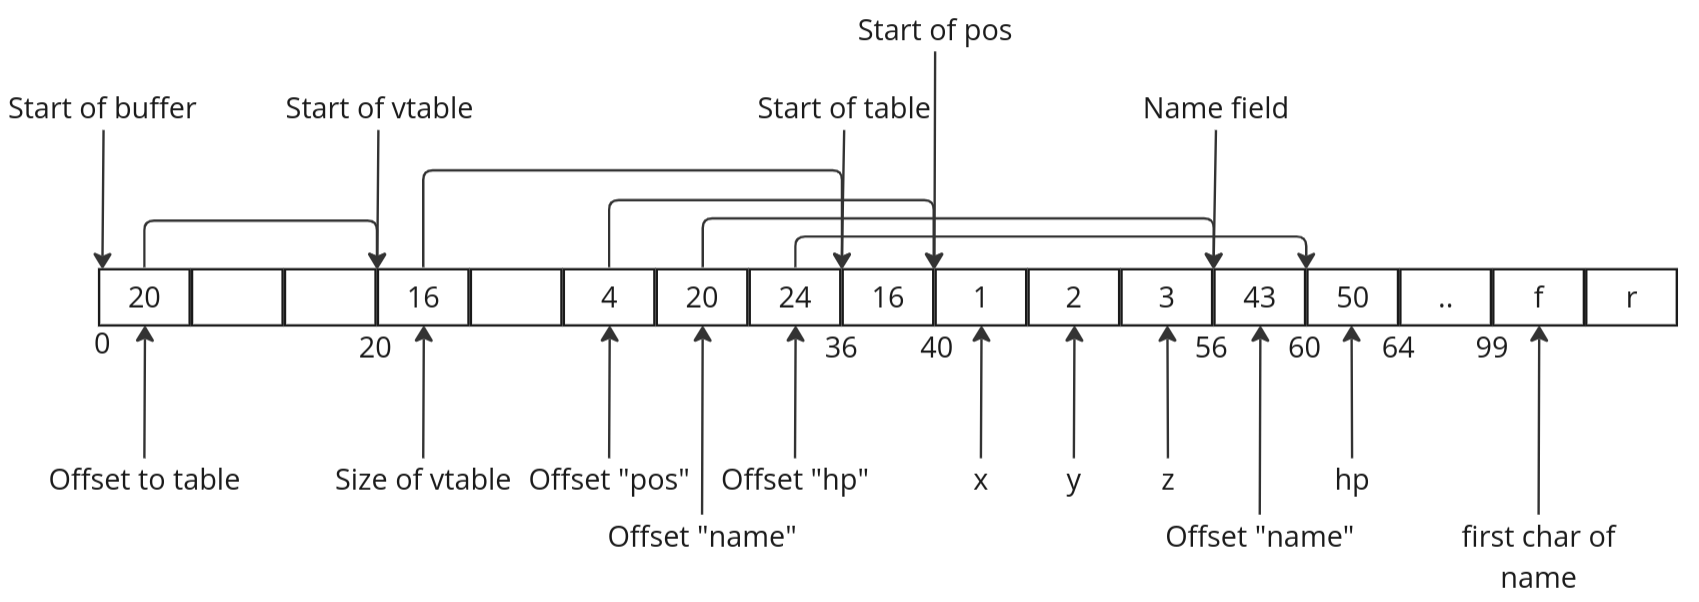
\includegraphics[width=\linewidth, height=7cm, keepaspectratio]{./figures/flatbuf.png}
    \caption{Flatbuffer structure showing offset pointers and values for the object \{ pos: \{ x: 1, y: 2, z: 3 \}, name: "fred", hp: 50 \}. The structures are marked by memory location in bytes.}
    \label{fig:flatbuf}
\end{figure}

\subsubsection{Packed Hilbert R-tree}
A Packed Hilbert R-tree is an extension of the R-tree, a balanced tree used for multidimensional data, in our case, spatial data. From \cite{rtree}, a regular R-tree stores all data as leaf nodes on the same level. All leaves have minimum bounding rectangles (MBRs) that geometrically contain the data element of that node. Parent nodes also have MBRs, MBRs of parents geoemtrically conatin all MBRs of the children. An example of this is shown in figure \ref{fig:rtree}, with the corresponding data in figure \ref{fig:mbrs}. This allows for efficient spatial queries. When querying with a spatial filter, the system will only explore nodes that have MBRs overlapping with the spatial filter. For large datasets, this can lead to significant performance gains for many queries, as much fewer nodes need to be accessed.

\begin{figure}
    \centering
    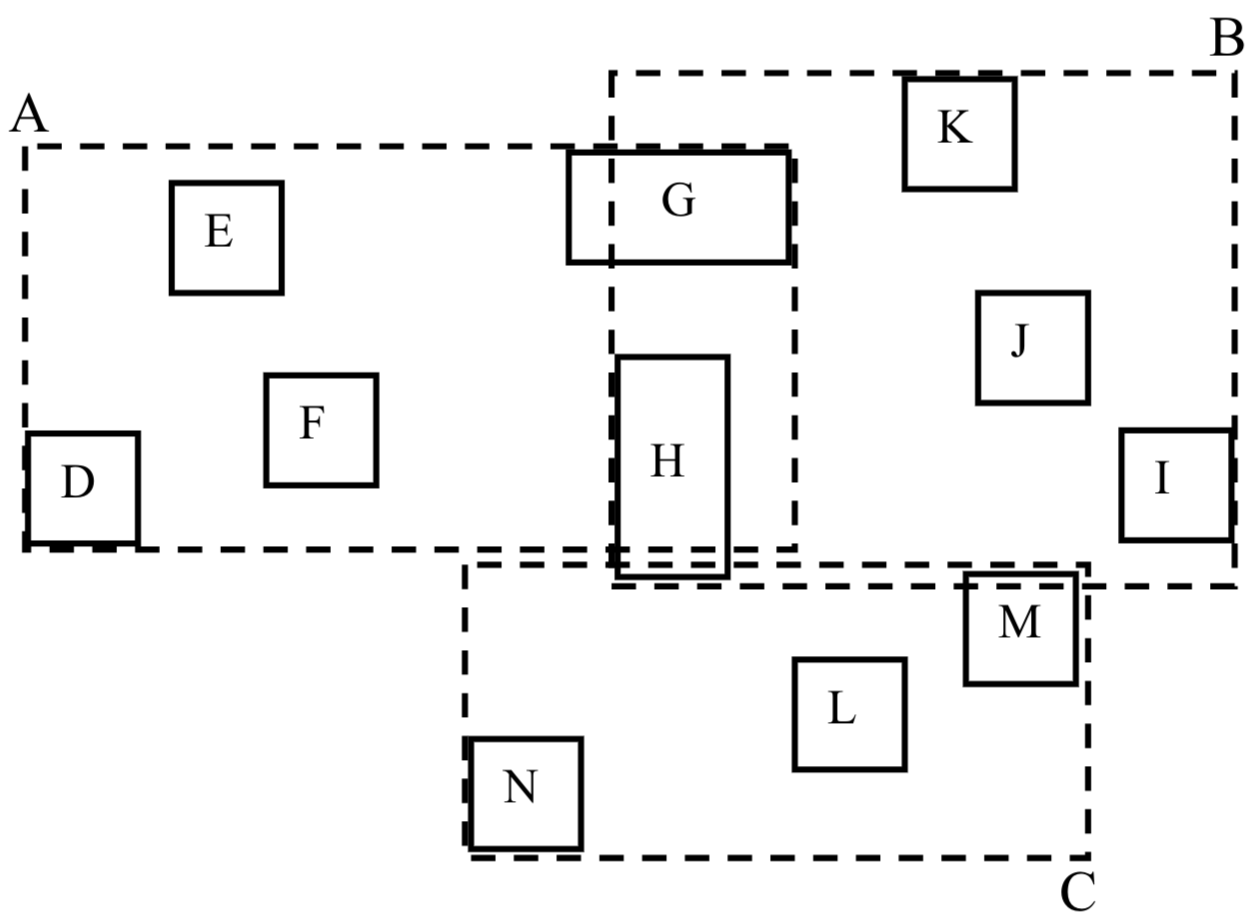
\includegraphics[width=0.5\linewidth]{./figures/mbrs.png}
    \caption{An example of data MBRs and their MBRs, from \cite{rtree}.}
    \label{fig:mbrs}
\end{figure}
\begin{figure}
    \centering
    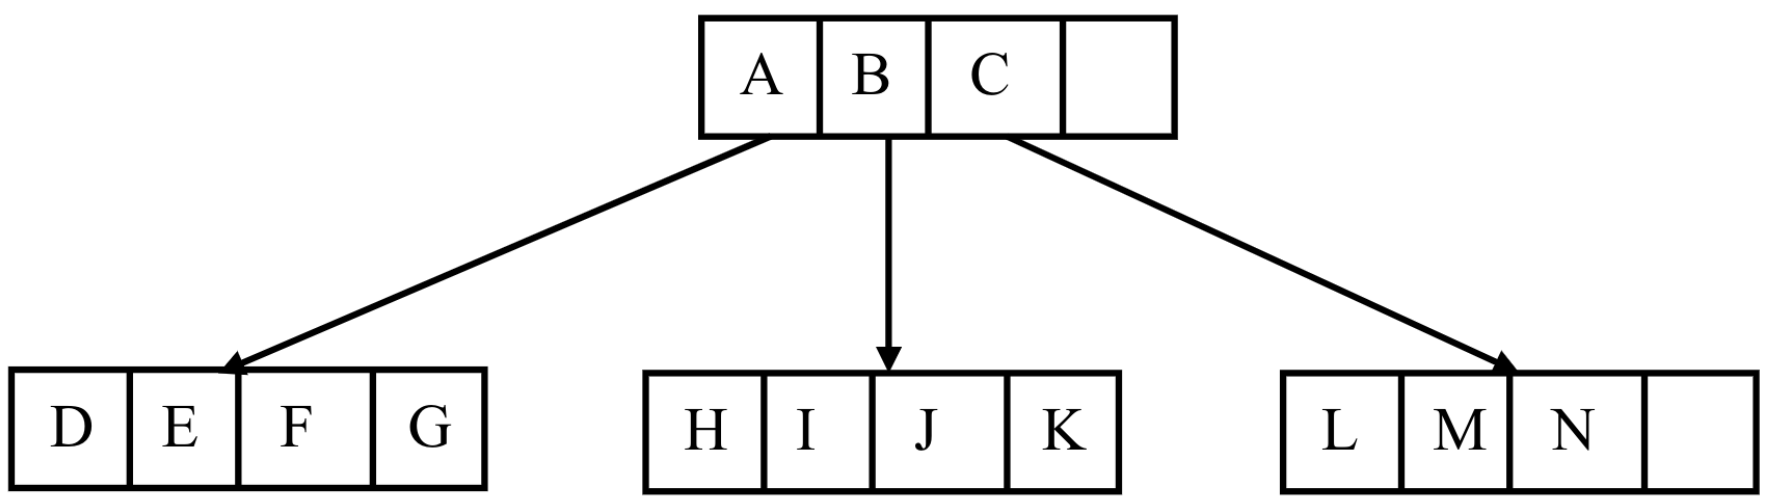
\includegraphics[width=\linewidth]{./figures/rtree.png}
    \caption{The corresponding R-tree, from \cite{rtree}.}
    \label{fig:rtree}
\end{figure}

What distinguishes a normal R-tree from a Hilbert R-tree is the MBR selection. The Hilbert R-tree utilizes Hilbert curves to generate MBRs for nodes. A Hilbert curve is a space-filling curve that can traverse every point in higher-dimensional space. This property allows for the mapping of two-dimensional values to one-dimensional values by drawing the curve in two dimensions and assigning ascending values to the points along the curve, see figure \ref{fig:hilbert} for Hilbert curves with corresponding values. These values are referred to as Hilbert values. Hilbert curves have the characteristic such that elements close in space will also be close in Hilbert values. By sorting MBRs based on the Hilbert value of the rectangle centroids, we can create MBRs with minimal overlap for spatial indexing.

\begin{figure}[t]
    \centering
    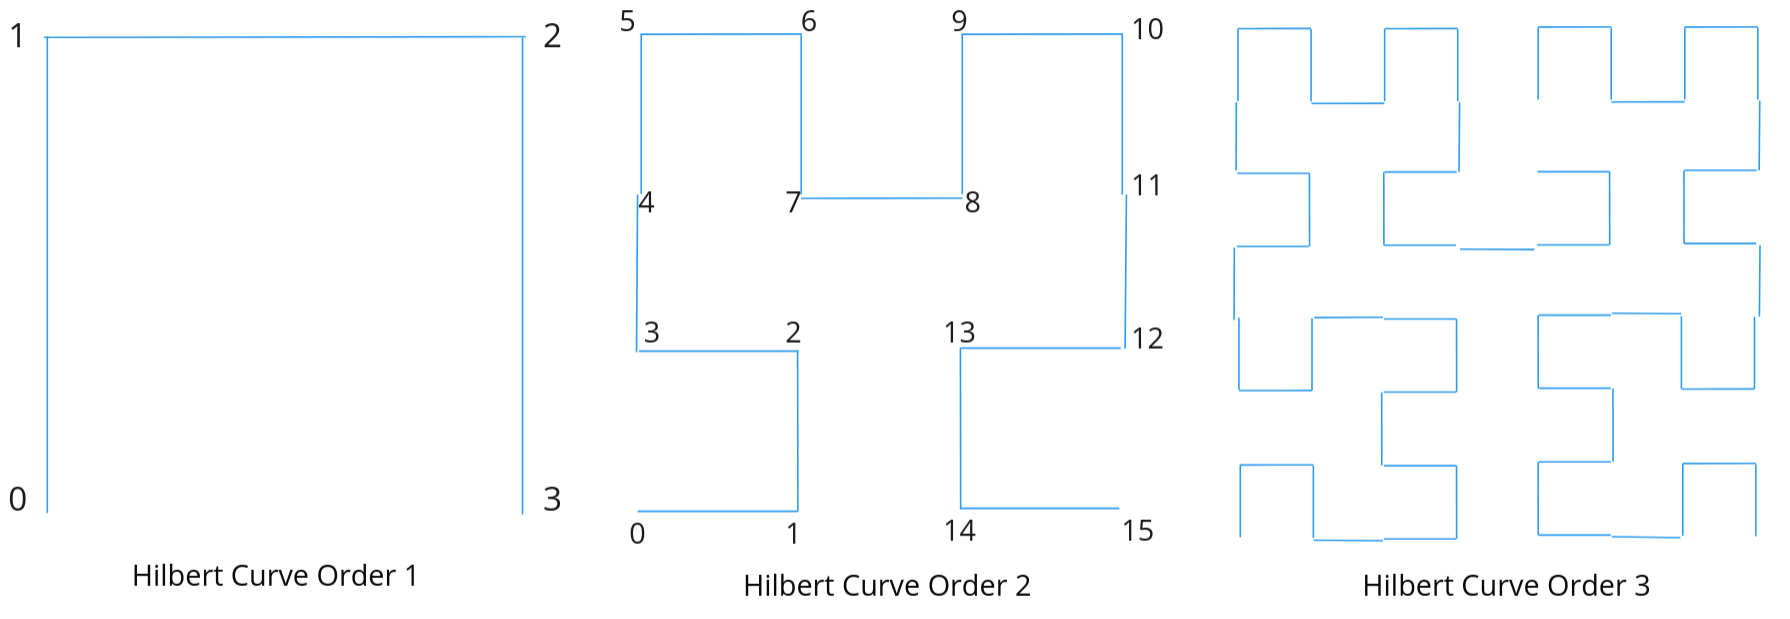
\includegraphics[width=\linewidth]{./figures/hilbert_orders.png}
    \caption{Showing Hilbert Curves of orders 1, 2, and 3.}
    \label{fig:hilbert}
\end{figure}

The Packed Hilbert R-tree is an optimized version of the Hilbert Tree. The Packed R-tree has even less overlap, resulting in improved query performance. The downside is that it requires more resources for construction. Considering the additional resource consumption, the Packed variant is only practical for applications that heavily prioritize read operations. In a system with frequent write operations, the entire tree would need to be rewritten frequently, leading to significant performance loss. For this reason, the Packed Hilbert R-tree is also known as the static Hilbert R-tree.

\subsubsection{FlatGeoBuf implementation}
Flatbuffers and Packed Hilbert R-trees are combined into a new format called FlatGeoBuf. The format consists of four parts, Magic Bytes, Header, R-tree index, and Data, see figure \ref{fig:fgb}. The Magic Bytes is used to identify which format the content is in (aka FGB), and specifies which major and minor version is currently begin used. The Header contains general metadata about the file, such as the filename, schemas, information about the index, coordinate reference system, and feature count. For homogoenous FGB files, files that only contain one geometry type or files where all features have the same schema, this schema is defined in the header instead of repeating it for every feature. For heterogenous FGB files this information will be stored on each feature. The indexing structure is a flattened packed Hilbert R-tree containing spatial indexes. If spatial indexing is disabled the Data section will appear directly after the header instead. The index is structured like an R-tree using buffers and offsets. All nodes in the index conatin an MBR and an offset. For tree nodes the offset points further down the tree, to another tree node or to a leaf node. For leaf nodes the offsets point to the actual data feature in the Data section.

The Features are the most complex part of the structure, since they can represent many different geometrie types while being very efficient. Features have the fields: $geometry$, $properties$, and $columns$. The essential fields of $geometry$ are: $xy$ and $type$. The latitude and longitude is stored in the same field $xy$, which is an array, to have a compact and flat structure. The even indexes are latitudes and odd indexes are longitudes. An example object of a LineString is $\{xy: [5, 6, 8, 9], type: 2\}$. This represents the line between the points $(5, 8)$ and $(6, 9)$, the coordinates are given by $xy$ and the type LineString is given by $type$.
\begin{figure}[h]
    \centering
    \begin{tikzpicture}
        % Define nodes with the correct keys
        \node [rectangle, draw, fill=blue!30,
            minimum width=0.1\linewidth, minimum height=1cm, label=center:MB] (mb) at (0,0) {};
        \node [rectangle, draw, fill=teal!30, right=0cm of mb,
            minimum width=0.19\linewidth, minimum height=1cm, label=center:H] (h) {};
        \node [rectangle, draw, fill=blue!30, right=0cm of h,
            minimum width=0.19\linewidth, minimum height=1cm, label=center:I] (i) {};
        \node [rectangle, draw, fill=teal!30, right=0cm of i,
            minimum width=0.5\linewidth, minimum height=1cm, label=center:DATA] (data) {};
    \end{tikzpicture}
    \begin{itemize}
        \item \textbf{MB}: Magic Bytes (uniquely identify the file format)
        \item \textbf{H}: Header (varaible size flatbuffer)
        \item \textbf{I} (Optional): Static Packed Hilbert R-tree index (static size custom buffer)
        \item \textbf{DATA}: Features (variable size flatbuffer)
    \end{itemize}
    \caption{ FlatGeoBufs internal structure, from \cite{fgb_org}. }
    \label{fig:fgb}
\end{figure}

\subsubsection{FGBs benefits for HTTP}
The FGB format is excellent for use across HTTP using range requests. This is because the index and data structure allows for the data to be lazily loaded. Furthermore, this allows the data to be streamed for more efficient loading. Another reason why this is important is that many Big Data operations take place in the so called "cloud-native" environment. Meaning it is built only to exist in the cloud. In these environemnts you typically use large partitioned files. FGB is optimal for use in cloud-native environments.

\subsection{GeoJSON}
GeoJSON was released in 2016 as a subset of JSON intented for use in web development. It consists of key-value pairs like in JSON, but they are limited to the properties of simple geographical features. The features include: points, linestrings, polygons among other things, see figure \ref{fig:geojson} for and example LineString.

\begin{figure}[h]
    \begin{verbatim}
    {
        "type": "LineString", 
        "coordinates": [
            [63.449, 10.438],
            [63.442, 10.437],
            [63.437, 10.434],
            [63.42, 10.439],
        ]
    }
\end{verbatim}
    \caption{Example of a GeoJSON LineString object.}
    \label{fig:geojson}
\end{figure}
For the purposes of this thesis GeoJSON has most specification requirements covered, and mainly lacks in performance. The major issue for Big Data use, arises from its verbose structure which is required for human readability. It includes all field names and values, even for objects where the same schema is repeated thousands of times. Additionally it includes unnecessary padding and whitespaces. This is included to simplifiy web deveolpment as developers can easily understand the document and edit it directly. On the other hand it bloats file- and transmission sizes. Sacrificing size for human readability provides little to no benefit for Big Data operations.

Json serialization is also slow because of its flexibility. The JSON serializer performs analysis on the data in order to determine the data type, int / object / string, this is inefficient. In addition GeoJSON allows deeply nested and complex structures which will furher slow down parsing.

\subsection{Shapefile}
The Shapefile format was released as the official format for geospatial data by the Open Geospatial Consortium (OGC) in 1998. Eventhough it was officially replaced by GeoPackage in 2014, the Shapefile is still in widespread use. It is a multifile format, meaning when it is created the data and meta data is split into different files. The main file is the .shp file, which contains the geometry data. Another essential generated file is the .shx file, which contains the indexes to the features. Although this format is old, there are many benefits in using it. The format is widely supported as it was the first officially supported format and was the industry standard for a long time. In addition, the .shx and .shp file enables efficient reading. In terms of file size it outcompetes text based formats like GeoJSON.

However, there are also major drawbacks, the file size is limited to 2GB, and the format requires multiple files. Additionally there is no official support for 3D data. The format has no support for hierarchies or trees either, making the storage of complex geometrical features impossible. All in all the Shapefile should prefferably not be used, but it does work for some simple projects. Choosing Shapefile as a format might also be easier in certain scenarious due to its widespread support.
